\chapter{深入理解程序的执行}
\section{pyc 文件结构}
在本小节当中主要给大家介绍一下 .py 文件在被编译之后对应的 pyc 文件结构,pyc 文件当中的一个核心内容就是 python 字节码。
\subsection{pyc 文件}
pyc 文件是 Python 在解释执行源代码时生成的一种字节码文件,它包含了源代码的编译结果和相关的元数据信息,以便于 Python 可以更快地加载和执行代码。
Python 是一种解释型语言,它不像编译型语言那样将源代码直接编译成机器码执行。Python 的解释器会在运行代码之前先将源代码编译成字节码,然后将字节码解释执行。.pyc 文件就是这个过程中生成的字节码文件。
当 Python 解释器首次执行一个 .py 文件时,它会在同一目录下生成一个对应的 .pyc 文件,以便于下次加载该文件时可以更快地执行。如果源文件在修改之后被重新加载,解释器会重新生成 .pyc 文件以更新缓存的字节码。
\subsection{生成 pyc 文件}
正常的 python 文件需要通过编译器变成字节码,然后将字节码交给 python 虚拟机,然后 python 虚拟机会执行字节码。整体流程如下所示:

    \begin{figure}[H]
        \centering
            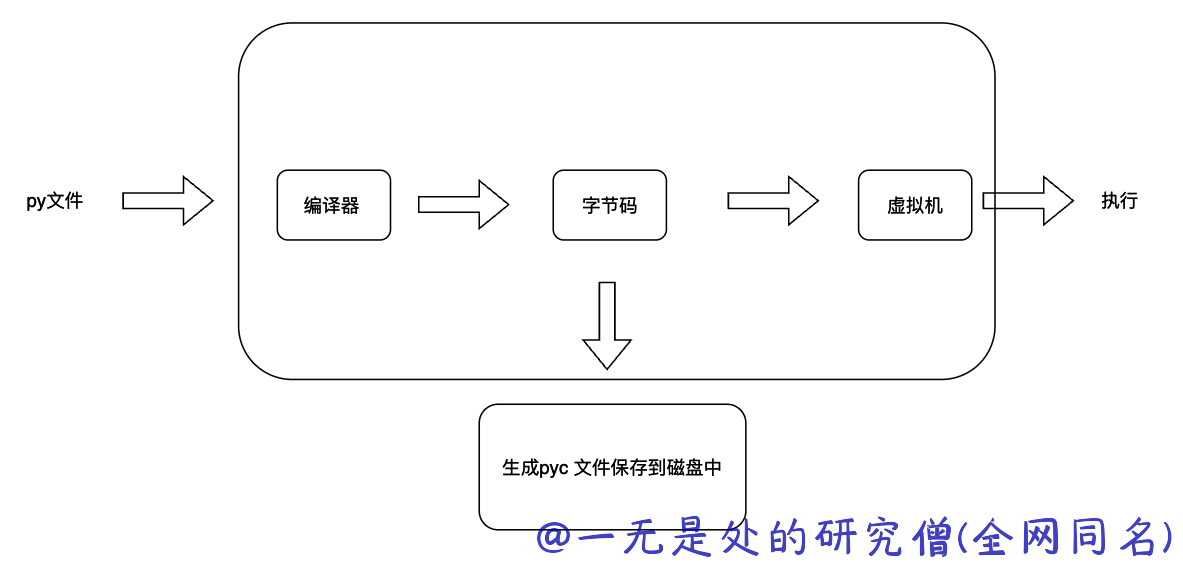
\includegraphics[scale=.25]{images/35-pyc.png}
						\caption{ }
        \label{fig:my_label}
    \end{figure}
    
我们可以直接使用 compile all 模块生成对应文件的 pyc 文件。
\begin{lstlisting}[style=cpp,caption=, language=C++]

➜  pvm ls
demo.py  hello.py
➜  pvm python -m compileall .
Listing '.'...
Listing './.idea'...
Listing './.idea/inspectionProfiles'...
Compiling './demo.py'...
Compiling './hello.py'...
➜  pvm ls
__pycache__ demo.py     hello.py
➜  pvm ls __pycache__ 
demo.cpython-310.pyc  hello.cpython-310.pyc
\end{lstlisting}
\verb|python -m compileall .| 命令将递归扫描当前目录下面的 py 文件,并且生成对应文件的 pyc 文件。
\subsection{pyc 文件布局}

    \begin{figure}[H]
        \centering
            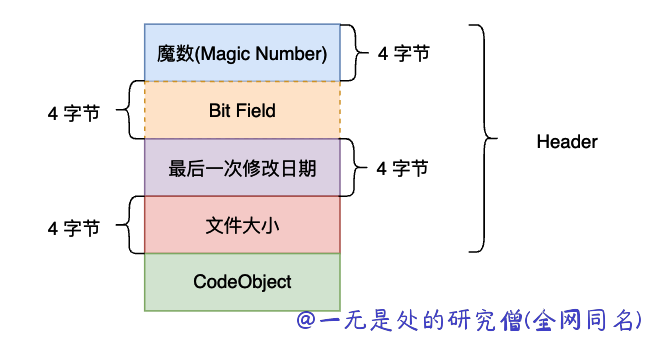
\includegraphics[scale=.35]{images/38-pyc.png}
						\caption{ }
        \label{fig:my_label}
    \end{figure}
    
第一部分魔数由两部分组成:

    \begin{figure}[H]
        \centering
            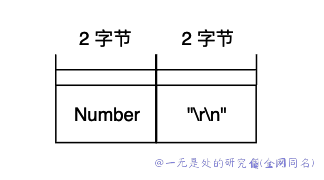
\includegraphics[scale=.3]{images/37-pyc.png}
						\caption{ }
        \label{fig:my_label}
    \end{figure}
第一部分 魔术是由一个 2 字节的整数和另外两个字符回车换行组成的, \verb|"\r\n"|  也占用两个字节,一共是四个字节。这个两个字节的整数在不同的 python 版本还不一样,比如说在 python3.5 当中这个值为 3351 等值,在 python3.9 当中这个值为 3420,3421,3422,3423,3424等值(在 python 3.9 的小版本)。

第二部分 Bit Field 这个字段的主要作用是为了将来能够实现复现编译结果,但是在 python3.9a2 时,这个字段的值还全部是 0 。详细内容可以参考 [PEP552-Deterministic pycs]\footnote{\href{https://peps.python.org/pep-0552/}{https://peps.python.org/pep-0552/}} 。这个字段在 python2 和 python3 早期版本并没有(python3.5 还没有),在 python3 的后期版本这个字段才出现的。

第三部分 就是整个 py  源文件的大小了。

第四部分 也是整个 pyc 文件当中最重要的一个部分,最后一个部分就是一个 CodeObject 对象序列化之后的数据,我们稍后再来仔细分析一下这个对象相关的数据。

我们现在来具体分析一个 pyc 文件,对应的 python 代码为:
\begin{lstlisting}[style=py,caption=, language=Python]

def f():
    x = 1
    return 2
\end{lstlisting}
pyc 文件的十六进制形式如下所示:
\begin{lstlisting}[style=cpp,caption=, language=C++]

➜  __pycache__ hexdump -C hello.cpython-310.pyc
00000000  6f 0d 0d 0a 00 00 00 00  b9 48 21 64 20 00 00 00  |o........H!d ...|
00000010  e3 00 00 00 00 00 00 00  00 00 00 00 00 00 00 00  |................|
00000020  00 02 00 00 00 40 00 00  00 73 0c 00 00 00 64 00  |.....@...s....d.|
00000030  64 01 84 00 5a 00 64 02  53 00 29 03 63 00 00 00  |d...Z.d.S.).c...|
00000040  00 00 00 00 00 00 00 00  00 01 00 00 00 01 00 00  |................|
00000050  00 43 00 00 00 73 08 00  00 00 64 01 7d 00 64 02  |.C...s....d.}.d.|
00000060  53 00 29 03 4e e9 01 00  00 00 e9 02 00 00 00 a9  |S.).N...........|
00000070  00 29 01 da 01 78 72 03  00 00 00 72 03 00 00 00  |.)...xr....r....|
00000080  fa 0a 2e 2f 68 65 6c 6c  6f 2e 70 79 da 01 66 01  |.hello.py..f.|
00000090  00 00 00 73 04 00 00 00  04 01 04 01 72 06 00 00  |...s........r...|
000000a0  00 4e 29 01 72 06 00 00  00 72 03 00 00 00 72 03  |.N).r....r....r.|
000000b0  00 00 00 72 03 00 00 00  72 05 00 00 00 da 08 3c  |...r....r......<|
000000c0  6d 6f 64 75 6c 65 3e 01  00 00 00 73 02 00 00 00  |module>....s....|
000000d0  0c 00                                             |..|
000000d2
\end{lstlisting}
因为数据使用小端表示方式,因此对于上面的数据来说:
\begin{itemize}
\item 第一部分魔数为:0xa0d0d6f 。 
\item 第二部分 Bit Field 为:0x0 。 
\item 第三部分最后一次修改日期为:0x642148b9 。 
\item 第四部分文件大小为:0x20 字节,也就是说 hello.py 这个文件的大小是 32 字节。 
\end{itemize}
下面是一个小的代码片段用于读取 pyc 文件的头部元信息:
\begin{lstlisting}[style=py,caption=, language=Python]

import struct
import time
import binascii
fname = "./__pycache__/hello.cpython-310.pyc"
f = open(fname, "rb")
magic = struct.unpack('<l', f.read(4))[0]
bit_filed = f.read(4)
print(f"bit field = {binascii.hexlify(bit_filed)}")
moddate = f.read(4)
filesz = f.read(4)
modtime = time.asctime(time.localtime(struct.unpack('<l', moddate)[0]))
filesz = struct.unpack('<L', filesz)
print("magic %s" % (hex(magic)))
print("moddate (%s)" % (modtime))
print("File Size %d" % filesz)
f.close()
\end{lstlisting}
上面的代码输出结果如下所示:
\begin{lstlisting}[style=cpp,caption=, language=C++]

bit field = b'00000000'
magic 0xa0d0d6f
moddate (Mon Mar 27 15:41:45 2023)
File Size 32
\end{lstlisting}
有关 pyc 文件的详细操作可以查看 python 标准库 importlib/\_bootstrap\_external.py 文件源代码。
\subsection{CodeObject}
在 CPython 中,\verb|CodeObject| 是一个对象,它包含了 Python 代码的字节码、常量、变量、位置参数、关键字参数等信息,以及一些用于运行代码的元数据,如文件名、代码行号等。
在 CPython 中,当我们执行一个 Python 模块或函数时,解释器会先将其代码编译为 \verb|CodeObject|,然后再执行。在编译过程中,解释器会将 Python 代码转换为字节码,并将其保存在 \verb|CodeObject| 对象中。此后,每当我们调用该模块或函数时,解释器都会使用 \verb|CodeObject| 中的字节码来执行代码。
\verb|CodeObject| 对象是不可变的,一旦创建就不能被修改。这是因为 Python 代码的字节码是不可变的,而 \verb|CodeObject| 对象包含了这些字节码,所以也是不可变的。
在本小节当中主要介绍 code object 当中主要的内容,以及简单介绍他们的作用,在后续的文章当中会仔细分析 code object 对应的源代码以及对应的字段的详细作用。
现在举一个例子来分析一下 pycdemo.py 的 pyc 文件,pycdemo.py 的源程序如下所示:
\begin{lstlisting}[style=py,caption=, language=Python]

if __name__ == '__main__':
    a = 100
    print(a)
\end{lstlisting}
下面的代码是一个用于加载 pycdemo01.cpython-39.pyc 文件(也就是 hello.py 对应的 pyc 文件)的代码,使用 marshal 读取 pyc 文件里面的 code object 。
\begin{lstlisting}[style=py,caption=, language=Python]

import marshal
import dis
import struct
import time
import types
import binascii
def print_metadata(fp):
    magic = struct.unpack('<l', fp.read(4))[0]
    print(f"magic number = {hex(magic)}")
    bit_field = struct.unpack('<l', fp.read(4))[0]
    print(f"bit filed = {bit_field}")
    t = struct.unpack('<l', fp.read(4))[0]
    print(f"time = {time.asctime(time.localtime(t))}")
    file_size = struct.unpack('<l', fp.read(4))[0]
    print(f"file size = {file_size}")
def show_code(code, indent=''):
    print ("%scode" % indent)
    indent += '   '
    print ("%sargcount %d" % (indent, code.co_argcount))
    print ("%snlocals %d" % (indent, code.co_nlocals))
    print ("%sstacksize %d" % (indent, code.co_stacksize))
    print ("%sflags %04x" % (indent, code.co_flags))
    show_hex("code", code.co_code, indent=indent)
    dis.disassemble(code)
    print ("%sconsts" % indent)
    for const in code.co_consts:
        if type(const) == types.CodeType:
            show_code(const, indent+'   ')
        else:
            print("   %s%r" % (indent, const))
    print("%snames %r" % (indent, code.co_names))
    print("%svarnames %r" % (indent, code.co_varnames))
    print("%sfreevars %r" % (indent, code.co_freevars))
    print("%scellvars %r" % (indent, code.co_cellvars))
    print("%sfilename %r" % (indent, code.co_filename))
    print("%sname %r" % (indent, code.co_name))
    print("%sfirstlineno %d" % (indent, code.co_firstlineno))
    show_hex("lnotab", code.co_lnotab, indent=indent)
def show_hex(label, h, indent):
    h = binascii.hexlify(h)
    if len(h) < 60:
        print("%s%s %s" % (indent, label, h))
    else:
        print("%s%s" % (indent, label))
        for i in range(0, len(h), 60):
            print("%s   %s" % (indent, h[i:i+60]))
if __name__ == '__main__':
    filename = "./__pycache__/pycdemo01.cpython-39.pyc"
    with open(filename, "rb") as fp:
        print_metadata(fp)
        code_object = marshal.load(fp)
        show_code(code_object)
\end{lstlisting}
执行上面的程序输出结果如下所示:
\begin{lstlisting}[style=cpp,caption=, language=C++]

magic number = 0xa0d0d61
bit filed = 0
time = Tue Mar 28 02:40:20 2023
file size = 54
code
   argcount 0
   nlocals 0
   stacksize 2
   flags 0040
   code b'650064006b02721464015a01650265018301010064025300'
  3           0 LOAD_NAME                0 (__name__)
              2 LOAD_CONST               0 ('__main__')
              4 COMPARE_OP               2 (==)
              6 POP_JUMP_IF_FALSE       20
  4           8 LOAD_CONST               1 (100)
             10 STORE_NAME               1 (a)
  5          12 LOAD_NAME                2 (print)
             14 LOAD_NAME                1 (a)
             16 CALL_FUNCTION            1
             18 POP_TOP
        >>   20 LOAD_CONST               2 (None)
             22 RETURN_VALUE
   consts
      '__main__'
      100
      None
   names ('__name__', 'a', 'print')
   varnames ()
   freevars ()
   cellvars ()
   filename './pycdemo01.py'
   name '<module>'
   firstlineno 3
   lnotab b'08010401'
\end{lstlisting}
下面是 code object 当中各个字段的作用:
\begin{itemize}
\item 首先需要了解一下代码块这个概念,所谓代码块就是一个小的 python 代码,被当做一个小的单元整体执行。在 python 当中常见的代码块块有:函数体、类的定义、一个模块。 
\item argcount,这个表示一个代码块的参数个数,这个参数只对函数体代码块有用,因为函数可能会有参数,比如上面的 pycdemo.py 是一个模块而不是一个函数,因此这个参数对应的值为 0 。 
\item co\_code,这个对象的具体内容就是一个字节序列,存储真实的 python 字节码,主要是用于 python 虚拟机执行的,在本小节当中暂时不详细分析。 
\item co\_consts,这个字段是一个列表类型的字段,主要是包含一些字符串常量和数值常量,比如上面的 "\_\_main\_\_" 和 100 。 
\item co\_filename,这个字段的含义就是对应的源文件的文件名。 
\item co\_firstlineno,这个字段的含义为在 python 源文件当中第一行代码出现的行数,这个字段在进行调试的时候非常重要。 
\item co\_flags,这个字段的主要含义就是标识这个 code object 的类型。0x0080 表示这个 block 是一个协程,0x0010 表示这个 code object 是嵌套的等等。 
\item co\_lnotab,这个字段的含义主要是用于计算每个字节码指令对应的源代码行数。 
\item co\_varnames,这个字段的主要含义是表示在一个 code object 本地定义的一个名字。 
\item co\_names,和 co\_varnames 相反,表示非本地定义但是在 code object 当中使用的名字。 
\item co\_nlocals,这个字段表示在一个 code object 当中本地使用的变量个数。 
\item co\_stackszie,因为 python 虚拟机是一个栈式计算机,这个参数的值表示这个栈需要的最大的值。 
\item co\_cellvars,co\_freevars,这两个字段主要和嵌套函数和函数闭包有关,我们在后续的文章当中将详细解释这个字段。 
\end{itemize}
\subsection{总结}
在本小节当中主要给大家介绍了 python 文件被编译之后的结果文件 .pyc 文件结构,在 pyc 文件当中一个最重要的结构就是 code object 对象,在本小节当中主要是简单介绍了 code object 各个字段的作用。在后续的文章当中将会举详细的例子进行说明,正确理解这些这些字段的含义,对于我们理解 python 虚拟机大有裨益。


\section{深入理解 python 虚拟机:字节码灵魂——Code obejct}
在本小节当中主要给大家深入介绍在 cpython 当中非常重要的一个数据结构 code object!在本小节当中将会举一些例子以便更加深入理解这些字段。
\subsection{Code Object 数据结构}
\begin{lstlisting}[style=cpp,caption=, language=C++]

typedef struct {
    PyObject_HEAD
    int co_argcount;		/* #arguments, except *args */
    int co_kwonlyargcount;	/* #keyword only arguments */
    int co_nlocals;		/* #local variables */
    int co_stacksize;		/* #entries needed for evaluation stack */
    int co_flags;		/* CO_..., see below */
    PyObject *co_code;		/* instruction opcodes */
    PyObject *co_consts;	/* list (constants used) */
    PyObject *co_names;		/* list of strings (names used) */
    PyObject *co_varnames;	/* tuple of strings (local variable names) */
    PyObject *co_freevars;	/* tuple of strings (free variable names) */
    PyObject *co_cellvars;      /* tuple of strings (cell variable names) */
    /* The rest aren't used in either hash or comparisons, except for
       co_name (used in both) and co_firstlineno (used only in
       comparisons).  This is done to preserve the name and line number
       for tracebacks and debuggers; otherwise, constant de-duplication
       would collapse identical functions/lambdas defined on different lines.
    */
    unsigned char *co_cell2arg; /* Maps cell vars which are arguments. */
    PyObject *co_filename;	/* unicode (where it was loaded from) */
    PyObject *co_name;		/* unicode (name, for reference) */
    int co_firstlineno;		/* first source line number */
    PyObject *co_lnotab;	/* string (encoding addr<->lineno mapping) See
				   Objects/lnotab_notes.txt for details. */
    void *co_zombieframe;     /* for optimization only (see frameobject.c) */
    PyObject *co_weakreflist;   /* to support weakrefs to code objects */
} PyCodeObject;
\end{lstlisting}
下面是 code object 当中各个字段的作用:
\begin{itemize}
\item 首先需要了解一下代码块这个概念,所谓代码块就是一个小的 python 代码,被当做一个小的单元整体执行。在 python 当中常见的代码块块有:函数体、类的定义、一个模块。 
\item argcount,这个表示一个代码块的参数个数,这个参数只对函数体代码块有用,因为函数可能会有参数,比如上面的 pycdemo.py 是一个模块而不是一个函数,因此这个参数对应的值为 0 。 
\item co\_code,这个对象的具体内容就是一个字节序列,存储真实的 python 字节码,主要是用于 python 虚拟机执行的,在本小节当中暂时不详细分析。 
\item co\_consts,这个字段是一个列表类型的字段,主要是包含一些字符串常量和数值常量,比如上面的 "\_\_main\_\_" 和 100 。 
\item co\_filename,这个字段的含义就是对应的源文件的文件名。 
\item co\_firstlineno,这个字段的含义为在 python 源文件当中第一行代码出现的行数,这个字段在进行调试的时候非常重要。 
\item co\_flags,这个字段的主要含义就是标识这个 code object 的类型。0x0080 表示这个 block 是一个协程,0x0010 表示这个 code object 是嵌套的等等。 
\item co\_lnotab,这个字段的含义主要是用于计算每个字节码指令对应的源代码行数。 
\item co\_varnames,这个字段的主要含义是表示在一个 code object 本地定义的一个名字。 
\item co\_names,和 co\_varnames 相反,表示非本地定义但是在 code object 当中使用的名字。 
\item co\_nlocals,这个字段表示在一个 code object 当中本地使用的变量个数。 
\item co\_stackszie,因为 python 虚拟机是一个栈式计算机,这个参数的值表示这个栈需要的最大的值。 
\item co\_cellvars,co\_freevars,这两个字段主要和嵌套函数和函数闭包有关,我们在后续的文章当中将详细解释这个字段。 
\end{itemize}
\subsection{	CodeObject 详细分析}
现在我们使用一些实际的例子来分析具体的 code object 。
\begin{lstlisting}[style=py,caption=, language=Python]

import dis
import binascii
import types
d = 10
def test_co01(c):
    a = 1
    b = 2
    return a + b + c + d
\end{lstlisting}
在前面的文章当中我们提到过一个函数是包括一个 code object 对象,test\_co01 的 code object 对象的输出结果(完整代码见[co01](https://github.com/Chang-LeHung/dive-into-cpython/blob/master/code/codeobject/co01.py))如下所示:
\begin{lstlisting}[style=cpp,caption=, language=C++]

code
   argcount 1
   nlocals 3
   stacksize 2
   flags 0043 0x43
   code b'6401007d01006402007d02007c01007c0200177c0000177400001753'
  9           0 LOAD_CONST               1 (1)
              3 STORE_FAST               1 (a)
 10           6 LOAD_CONST               2 (2)
              9 STORE_FAST               2 (b)
 11          12 LOAD_FAST                1 (a)
             15 LOAD_FAST                2 (b)
             18 BINARY_ADD
             19 LOAD_FAST                0 (c)
             22 BINARY_ADD
             23 LOAD_GLOBAL              0 (d)
             26 BINARY_ADD
             27 RETURN_VALUE
   consts
      None
      1
      2
   names ('d',)
   varnames ('c', 'a', 'b')
   freevars ()
   cellvars ()
   filename '/tmp/pycharm_project_396/co01.py'
   name 'test_co01'
   firstlineno 8
   lnotab b'000106010601'
\end{lstlisting}
\begin{itemize}
\item 字段 argcount 的值等于 1,说明函数有一个参数,这个函数 test\_co01 有一个参数 c 是相互对应的。 
\item 字段 nlocals 的值等于 3,说明在函数 test\_co01 当中一个一共实现了三个函数本地变量 a, b, c 。 
\item 字段 names,对应代码代码当中的 co\_names,根据前面的定义就是 d 这个全局变量在函数  test\_co01 当中使用,但是却没有在函数当中定义了。 
\item 字段 varnames,这个就表示在本地定义使用的变量了,在函数 test\_co01 当中主要有三个变量 a, b, c 。 
\item 字段 filename,就是 python 文件的地址了。 
\item 字段 firstlineno 说明函数的第一行出现在对应 python 代码的 第 8 行。 
\end{itemize}
\subsubsection{Flags 字段详细分析}
我们具体使用 python3.5 的源代码进行分析,在 cpython 虚拟机的具体实现如下所示(Include/code.h):
\begin{lstlisting}[style=cpp,caption=, language=C++]

/* Masks for co_flags above */
#define CO_OPTIMIZED	0x0001
#define CO_NEWLOCALS	0x0002
#define CO_VARARGS	0x0004
#define CO_VARKEYWORDS	0x0008
#define CO_NESTED       0x0010
#define CO_GENERATOR    0x0020
/* The CO_NOFREE flag is set if there are no free or cell variables.
   This information is redundant, but it allows a single flag test
   to determine whether there is any extra work to be done when the
   call frame it setup.
*/
#define CO_NOFREE       0x0040
/* The CO_COROUTINE flag is set for coroutine functions (defined with
   async def keywords) */
#define CO_COROUTINE            0x0080
#define CO_ITERABLE_COROUTINE   0x0100
\end{lstlisting}
如果 flags 字段和上面的各个宏定义进行 \& 运算,如果得到的结果大于 0,则说明符合对应的条件。
上面的宏定义的含义如下所示:
\begin{itemize}
\item CO\_OPTIMIZED,这个字段表示 code object 是被优化过的,使用函数本地定义的变量。 
\item CO\_NEWLOCALS,这个字段的含义为当这个 code object 的代码被执行的时候会给栈帧当中的 f\_locals 对象创建一个 dict 对象。 
\item CO\_VARARGS,表示这个 code object 对象是否含有位置参数。 
\item CO\_VARKEYWORDS,表示这个 code object 是否含有关键字参数。 
\item CO\_NESTED,表示这个 code object 是一个嵌套函数。 
\item CO\_GENERATOR,表示这个 code object 是一个生成器。 
\item CO\_COROUTINE,表示这个 code object 是一个协程函数。 
\item CO\_ITERABLE\_COROUTINE,表示 code object 是一个可迭代的协程函数。 
\item CO\_NOFREE,这个表示没有 freevars 和 cellvars,即没有函数闭包。 
\end{itemize}
现在再分析一下前面的函数 test\_co01 的 flags,他对应的值等于 0x43,则说明这个函数满足三个特性分别是 CO\_NEWLOCALS,CO\_OPTIMIZED 和 CO\_NOFREE。
\subsubsection{freevars \& cellvars}
我们使用下面的函数来对这两个字段进行分析:
\begin{lstlisting}[style=py,caption=, language=Python]

def test_co02():
    a = 1
    b = 2
    def g():
        return a + b
    return a + b + g()
\end{lstlisting}
上面的函数的信息如下所示(完整代码见[co02](https://github.com/Chang-LeHung/dive-into-cpython/blob/master/code/codeobject/co01.py)):
\begin{lstlisting}[style=cpp,caption=, language=C++]

code
   argcount 0
   nlocals 1
   stacksize 3
   flags 0003 0x3
   code
      b'640100890000640200890100870000870100660200640300640400860000'
      b'7d0000880000880100177c00008300001753'
 15           0 LOAD_CONST               1 (1)
              3 STORE_DEREF              0 (a)
 16           6 LOAD_CONST               2 (2)
              9 STORE_DEREF              1 (b)
 18          12 LOAD_CLOSURE             0 (a)
             15 LOAD_CLOSURE             1 (b)
             18 BUILD_TUPLE              2
             21 LOAD_CONST               3 (<code object g at 0x7f133ff496f0, file "/tmp/pycharm_project_396/co01.py", line 18>)
             24 LOAD_CONST               4 ('test_co02.<locals>.g')
             27 MAKE_CLOSURE             0
             30 STORE_FAST               0 (g)
 20          33 LOAD_DEREF               0 (a)
             36 LOAD_DEREF               1 (b)
             39 BINARY_ADD
             40 LOAD_FAST                0 (g)
             43 CALL_FUNCTION            0 (0 positional, 0 keyword pair)
             46 BINARY_ADD
             47 RETURN_VALUE
   consts
      None
      1
      2
      code
         argcount 0
         nlocals 0
         stacksize 2
         flags 0013 0x13
         code b'8800008801001753'
 19           0 LOAD_DEREF               0 (a)
              3 LOAD_DEREF               1 (b)
              6 BINARY_ADD
              7 RETURN_VALUE
         consts
            None
         names ()
         varnames ()
         freevars ('a', 'b')
         cellvars ()
         filename '/tmp/pycharm_project_396/co01.py'
         name 'g'
         firstlineno 18
         lnotab b'0001'
      'test_co02.<locals>.g'
   names ()
   varnames ('g',)
   freevars ()
   cellvars ('a', 'b')
   filename '/tmp/pycharm_project_396/co01.py'
   name 'test_co02'
   firstlineno 14
   lnotab b'0001060106021502'
\end{lstlisting}
从上面的输出我们可以看到的是,函数 test\_co02 的 cellvars 为 ('a', 'b'),函数 g 的 freevars 为 ('a', 'b'),cellvars 表示在其他函数当中会使用本地定义的变量,freevars 表示本地会使用其他函数定义的变量。
再来分析一下函数 test\_co02 的 flags,他的 flags 等于 0x3 因为有闭包的存在因此 flags 不会存在 CO\_NOFREE,也就是少了值 0x0040 。
\subsubsection{stacksize}
这个字段存储的是在函数在被虚拟机执行的时候所需要的最大的栈空间的大小,这也是一种优化手段,因为在知道所需要的最大的栈空间,所以可以在函数执行的时候直接分配指定大小的空间不需要在函数执行的时候再去重新扩容。
\begin{lstlisting}[style=py,caption=, language=Python]

def test_stack():
    a = 1
    b = 2
    return a + b
\end{lstlisting}
上面的代码相关字节码等信息如下所示:
\begin{lstlisting}[style=cpp,caption=, language=C++]

code
   argcount 0
   nlocals 2
   stacksize 2
   flags 0043 0x43
   code b'6401007d00006402007d01007c00007c01001753'
   #					  字节码指令		 字节码指令参数  参数对应的值
 24           0 LOAD_CONST               1 (1)
              3 STORE_FAST               0 (a)
 25           6 LOAD_CONST               2 (2)
              9 STORE_FAST               1 (b)
 26          12 LOAD_FAST                0 (a)
             15 LOAD_FAST                1 (b)
             18 BINARY_ADD
             19 RETURN_VALUE
   consts
      None # 下标等于 0 的常量
      1 	# 下标等于 1 的常量
      2	   # 下标等于 2 的常量
   names ()
   varnames ('a', 'b')
   freevars ()
   cellvars ()
\end{lstlisting}
我们现在来模拟一下执行过程,在模拟之前我们首先来了解一下上面几条字节码的作用:
\begin{itemize}
\item LOAD\_CONST,将常量表当中的下标等于 i 个对象加载到栈当中,对应上面的代码  LOAD\_CONST 的参数 i = 1。因此加载测常量等于 1 。因此现在栈空间如下所示: 

    \begin{figure}[H]
        \centering
            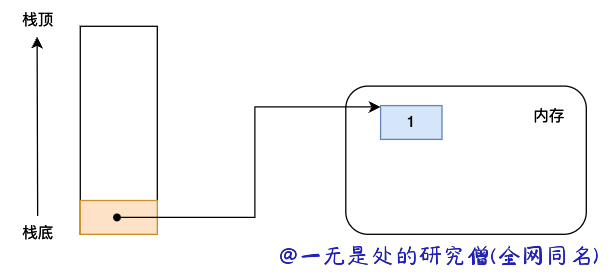
\includegraphics[scale=.2]{images/39-codeobject.png}
						\caption{ }
        \label{fig:my_label}
    \end{figure}
    
\item STORE\_FAST,将栈顶元素弹出并且保存到 co\_varnames 对应的下标当中,根据上面的字节码参数等于 0 ,因此将 1 保存到 co\_varnames[0] 对应的对象当中。 

    \begin{figure}[H]
        \centering
            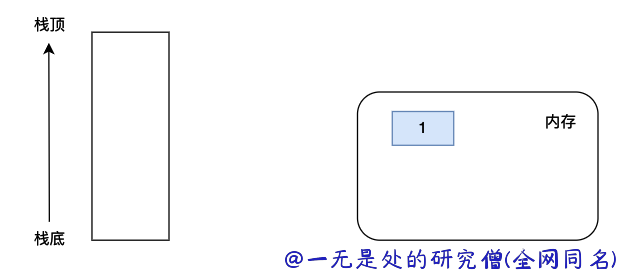
\includegraphics[scale=.2]{images/40-codeobject.png}
						\caption{ }
        \label{fig:my_label}
    \end{figure}
    
\item LOAD\_CONST,将下标等于 2 的常量加载进入栈中。 

    \begin{figure}[H]
        \centering
            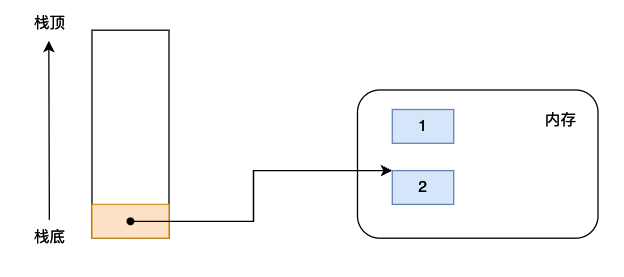
\includegraphics[scale=.2]{images/41-codeobject.png}
						\caption{ }
        \label{fig:my_label}
    \end{figure}
    
\item STORE\_FAST,将栈顶元素弹出,并且保存到 varnames 下标为 1 的对象。 

    \begin{figure}[H]
        \centering
            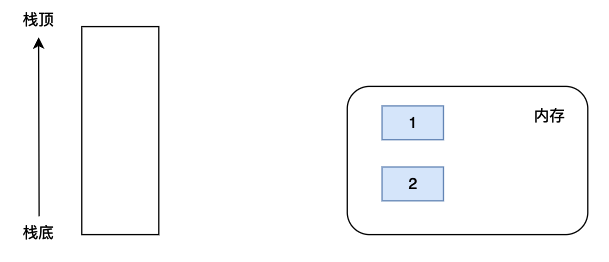
\includegraphics[scale=.2]{images/42-codeobject.png}
						\caption{ }
        \label{fig:my_label}
    \end{figure}
    
\item LOAD\_FAST,是取出 co\_varnames 对应下标的数据,并且将其压入栈中。我们直接连续执行两个 LOAD\_FAST 之后栈空间的布局如下: 

    \begin{figure}[H]
        \centering
            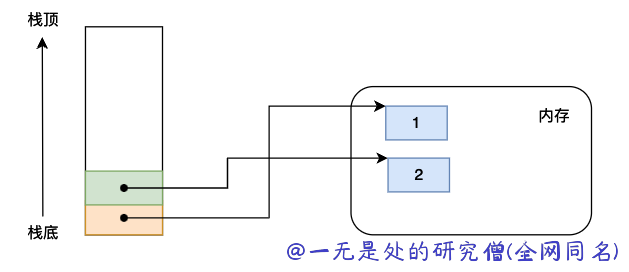
\includegraphics[scale=.2]{images/43-codeobject.png}
						\caption{ }
        \label{fig:my_label}
    \end{figure}
    
\item BINARY\_ADD,这个字节码指令是将栈空间的两个栈顶元素弹出,然后将两个数据进行相加操作,然后将相加得到的结果重新压入栈中。 

    \begin{figure}[H]
        \centering
            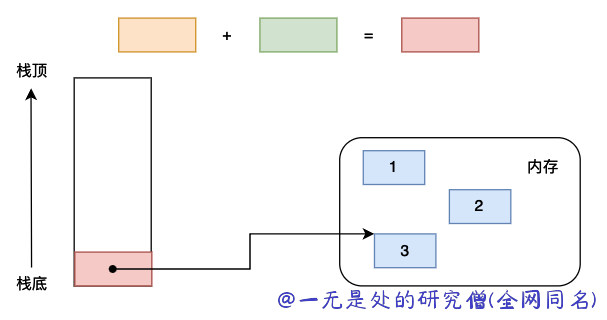
\includegraphics[scale=.2]{images/44-codeobject.png}
						\caption{ }
        \label{fig:my_label}
    \end{figure}
    
\item RETURN\_VALUE,将栈顶元素弹出并且作为返回值返回。 
\end{itemize}
从上面的整个执行过程来看整个栈空间使用的最大的空间长度为 2 ,因此 stacksize = 2 。
\subsection{总结}
在本小节当中主要分析了一些 code obejct 当中比较重要的字段,code object 是 cpython 虚拟机当中一个比较重要的数据结构,深入的去理解这里面的字段对于我们理解 python 虚拟机非常有帮助。

\section{深入理解 python 虚拟机:令人拍案叫绝的字节码设计}
在本小节当中主要给大家介绍 cpython 虚拟机对于字节码的设计以及在调试过程当中一个比较重要的字段 co\_lnotab 的设计原理!
\subsection{python 字节码设计}
一条 python 字节码主要有两部分组成,一部分是操作码,一部分是这个操作码的参数,在 cpython 当中只有部分字节码有参数,如果对应的字节码没有参数,那么 oparg 的值就等于 0 ,在 cpython 当中 opcode < 90 的指令是没有参数的。

    \begin{figure}[H]
        \centering
            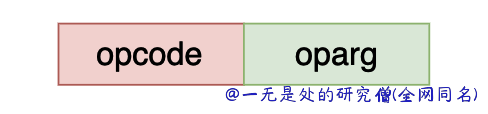
\includegraphics[scale=.25]{images/45-bytecode.png}
						\caption{ }
        \label{fig:my_label}
    \end{figure}

opcode 和 oparg 各占一个字节,cpython 虚拟机使用小端方式保存字节码。
我们使用下面的代码片段先了解一下字节码的设计:
\begin{lstlisting}[style=py,caption=, language=Python]

import dis
def add(a, b):
    return a + b
if __name__ == '__main__':
    print(add.__code__.co_code)
    print("bytecode: ", list(bytearray(add.__code__.co_code)))
    dis.dis(add)
\end{lstlisting}
上面的代码在 python3.9 的输出如下所示:
\begin{lstlisting}[style=cpp,caption=, language=C++]

b'|\x00|\x01\x17\x00S\x00'
bytecode:  [124, 0, 124, 1, 23, 0, 83, 0]
  5           0 LOAD_FAST                0 (a)
              2 LOAD_FAST                1 (b)
              4 BINARY_ADD
              6 RETURN_VALUE
\end{lstlisting}
首先 需要了解的是 \verb|add.__code__.co_code| 是函数 add 的字节码,是一个字节序列,\verb|list(bytearray(add.__code__.co_code))| 是将和这个序列一个字节一个字节进行分开,并且将其变成 10 进制形式。根据前面我们谈到的每一条指令——字节码占用 2 个字节,因此上面的字节码有四条指令:

    \begin{figure}[H]
        \centering
            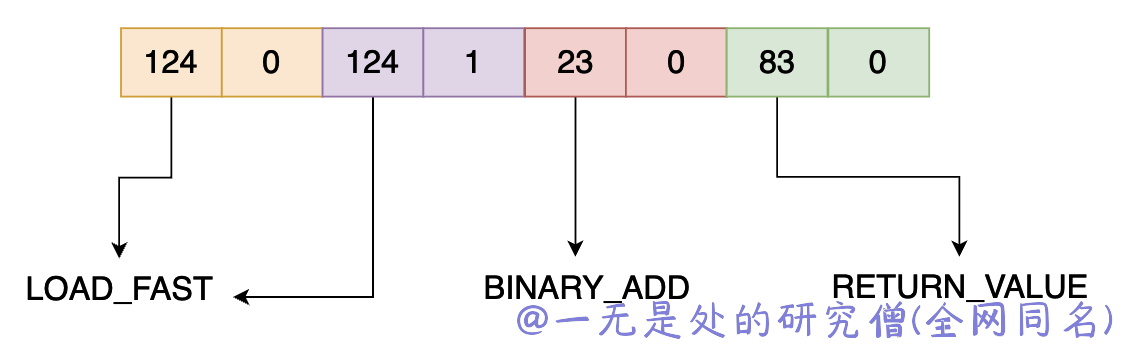
\includegraphics[scale=.25]{images/46-bytecode.png}
						\caption{ }
        \label{fig:my_label}
    \end{figure}

操作码和对应的操作指令在文末有详细的对应表。在上面的代码当中主要使用到了三个字节码指令分别是 124,23 和 83 ,他们对应的操作指令分别为 LOAD\_FAST,BINARY\_ADD,RETURN\_VALUE。他们的含义如下:
\begin{itemize}
\item LOAD\_FAST:将 varnames[var\_num] 压入栈顶。
\item BINARY\_ADD:从栈中弹出两个对象并且将它们相加的结果压入栈顶。
\item RETURN\_VALUE:弹出栈顶的元素,将其作为函数的返回值。
\end{itemize}
首先我们需要知道的是 BINARY\_ADD 和 RETURN\_VALUE,这两个操作指令是没有参数的,因此在这两个操作码之后的参数都是 0 。
但是 LOAD\_FAST 是有参数的,在上面我们已经知道 LOAD\_FAST 是将 co-varnames[var\_num] 压入栈,var\_num 就是指令 LOAD\_FAST 的参数。在上面的代码当中一共有两条 LOAD\_FAST 指令,分别是将 a 和 b 压入到栈中,他们在 varnames 当中的下标分别是 0 和 1,因此他们的操作数就是 0 和 1 。
\subsection{字节码扩展参数}
在上面我们谈到的 python 字节码操作数和操作码各占一个字节,但是如果 varnames 或者常量表的数据的个数大于 1 个字节的表示范围的话那么改如何处理呢?
为了解决这个问题,cpython 为字节码设计的扩展参数,比如说我们要加载常量表当中的下标为 66113 的对象,那么对应的字节码如下:
\begin{lstlisting}[style=py,caption=, language=Python]

[144, 1, 144, 2, 100, 65]
\end{lstlisting}
其中 144 表示 EXTENDED\_ARG,他本质上不是一个 python 虚拟机需要执行的字节码,这个字段设计出来主要是为了用与计算扩展参数的。
100 对应的操作指令是 LOAD\_CONST ,其操作码是 65,但是上面的指令并不会加载常量表当中下标为 65 对象,而是会加载下标为 66113 的对象,原因就是因为  EXTENDED\_ARG 。
现在来模拟一下上面的分析过程:
\begin{itemize}
\item 先读取一条字节码指令,操作码等于 144 ,说明是扩展参数,那么此时的参数 arg 就等于 (1 x (1 << 8)) = 256 。
\item 读取第二条字节码指令,操作码等于 144 ,说明是扩展参数,因为前面 arg 已经存在切不等于 0 了,那么此时 arg 的计算方式已经发生了改变,arg = arg << 8 + 2 << 8 ,也就是说原来的 arg 乘以 256 再加上新的操作数乘以 256 ,此时 arg = 66048 。
\item 读取第三条字节码指令,操作码等于 100,此时是 LOAD\_CONST 这条指令,那么此时的操作码等于 arg += 65,因为操作码不是 EXTENDED\_ARG 因此操作数不需要在乘以 256 了。
\end{itemize}
上面的计算过程用程序代码表示如下,下面的代码当中 code 就是真正的字节序列 HAVE\_ARGUMENT = 90 。
\begin{lstlisting}[style=py,caption=, language=Python]

def _unpack_opargs(code):
    extended_arg = 0
    for i in range(0, len(code), 2):
        op = code[i]
        if op >= HAVE_ARGUMENT:
            arg = code[i+1] | extended_arg
            extended_arg = (arg << 8) if op == EXTENDED_ARG else 0
        else:
            arg = None
        yield (i, op, arg)
\end{lstlisting}
我们可以使用代码来验证我们前面的分析:
\begin{lstlisting}[style=py,caption=, language=Python]

import dis
def num_to_byte(n):
    return n.to_bytes(1, "little")
def nums_to_bytes(data):
    ans = b"".join([num_to_byte(n) for n in data])
    return ans
if __name__ == '__main__':
    \section{extended_arg extended_num opcode oparg for python_version > 3.5}
    bytecode = nums_to_bytes([144, 1, 144, 2, 100, 65])
    print(bytecode)
    dis.dis(bytecode)
\end{lstlisting}
上面的代码输出结果如下所示:
\begin{lstlisting}[style=cpp,caption=, language=C++]

b'\x90\x01\x90\x02dA'
          0 EXTENDED_ARG             1
          2 EXTENDED_ARG           258
          4 LOAD_CONST           66113 (66113)
\end{lstlisting}
根据上面程序的输出结果可以看到我们的分析结果是正确的。
\subsection{源代码字节码映射表}
在本小节主要分析一个 code object 对象当中的 co\_lnotab 字段,通过分析一个具体的字段来学习这个字段的设计。
\begin{lstlisting}[style=py,caption=, language=Python]

import dis
def add(a, b):
    a += 1
    b += 2
    return a + b
if __name__ == '__main__':
    dis.dis(add.__code__)
    print(f"{list(bytearray(add.__code__.co_lnotab)) = }")
    print(f"{add.__code__.co_firstlineno = }")
\end{lstlisting}
首先 dis 的输出第一列是字节码对应的源代码的行号,第二列是字节码在字节序列当中的位移。
上面的代码输出结果如下所示:
\begin{lstlisting}[style=cpp,caption=, language=C++]

  源代码的行号  字节码的位移
  6           0 LOAD_FAST                0 (a)
              2 LOAD_CONST               1 (1)
              4 INPLACE_ADD
              6 STORE_FAST               0 (a)
  7           8 LOAD_FAST                1 (b)
             10 LOAD_CONST               2 (2)
             12 INPLACE_ADD
             14 STORE_FAST               1 (b)
  8          16 LOAD_FAST                0 (a)
             18 LOAD_FAST                1 (b)
             20 BINARY_ADD
             22 RETURN_VALUE
list(bytearray(add.__code__.co_lnotab)) = [0, 1, 8, 1, 8, 1]
add.__code__.co_firstlineno = 5
\end{lstlisting}
从上面代码的输出结果可以看出字节码一共分成三段,每段表示一行代码的字节码。现在我们来分析一下 co\_lnotab 这个字段,这个字段其实也是两个字节为一段的。比如上面的 [0, 1, 8, 1, 8, 1] 就可以分成三段 [0, 1], [8, 1], [8, 1] 。这其中的含义分别为:
\begin{itemize}
\item 第一个数字表示距离上一行代码的字节码数目。
\item 第二个数字表示距离上一行有效代码的行数。
\end{itemize}
现在我们来模拟上面代码的字节码的位移和源代码行数之间的关系:
\begin{itemize}
\item [0, 1],说明这行代码离上一行代码的字节位移是 0 ,因此我们可以看到使用 dis 输出的字节码 LOAD\_FAST ,前面的数字是 0,距离上一行代码的行数等于 1 ,代码的第一行的行号等于 5,因此 LOAD\_FAST 对应的行号等于 5 + 1 = 6 。
\item [8, 1],说明这行代码距离上一行代码的字节位移为 8 个字节,因此第二块的 LOAD\_FAST 前面是 8 ,距离上一行代码的行数等于 1,因此这个字节码对应的源代码的行号等于 6 + 1 = 7。
\item [8, 1],同理可以知道这块字节码对应源代码的行号是 8 。
\end{itemize}
现在有一个问题是当两行代码之间相距的行数超过 一个字节的表示范围怎么办?在 python3.5 以后如果行数差距大于 127,那么就使用 (0, 行数) 对下一个组合进行表示,(0, $x\_1$), (0,$ x\_2$) ... ,直到 $x\_1 + ... + x\_n$ = 行数。
在后面的程序当中我们会使用 compile 这个 python 内嵌函数。当你使用Python编写代码时,可以使用\verb|compile()|函数将Python代码编译成字节代码对象。这个字节码对象可以被传递给Python的解释器或虚拟机,以执行代码。
\verb|compile()|函数接受三个参数:
\begin{itemize}
\item \verb|source|: 要编译的Python代码,可以是字符串,字节码或AST对象。
\item \verb|filename|: 代码来源的文件名(如果有),通常为字符串。
\item \verb|mode|: 编译代码的模式。可以是 'exec'、'eval' 或 'single' 中的一个。'exec' 模式用于编译多行代码,'eval' 用于编译单个表达式,'single' 用于编译单行代码。
\end{itemize}
\begin{lstlisting}[style=py,caption=, language=Python]

import dis
code = """
x=1
y=2
""" \
+ "\n" * 500 + \
"""
z=x+y
"""
code = compile(code, '<string>', 'exec')
print(list(bytearray(code.co_lnotab)))
print(code.co_firstlineno)
dis.dis(code)
\end{lstlisting}
上面的代码输出结果如下所示:
\begin{lstlisting}[style=cpp,caption=, language=C++]

[0, 1, 4, 1, 4, 127, 0, 127, 0, 127, 0, 121]
1
  2           0 LOAD_CONST               0 (1)
              2 STORE_NAME               0 (x)
  3           4 LOAD_CONST               1 (2)
              6 STORE_NAME               1 (y)
505           8 LOAD_NAME                0 (x)
             10 LOAD_NAME                1 (y)
             12 BINARY_ADD
             14 STORE_NAME               2 (z)
             16 LOAD_CONST               2 (None)
             18 RETURN_VALUE
\end{lstlisting}
根据我们前面的分析因为第三行和第二行之间的差距大于 127 ,因此后面的多个组合都是用于表示行数的。
505 = 3(前面已经有三行了) + (127 + 127 + 127 + 121)(这个是第二行和第三行之间的差距,这个值为 502,中间有 500 个换行但是因为字符串相加的原因还增加了两个换行,因此一共是 502 个换行)。
具体的算法用代码表示如下所示,下面的参数就是我们传递给 dis 模块的 code,也就是一个 code object 对象。
\begin{lstlisting}[style=py,caption=, language=Python]

def findlinestarts(code):
    """Find the offsets in a byte code which are start of lines in the source.
    Generate pairs (offset, lineno) as described in Python/compile.c.
    """
    byte_increments = code.co_lnotab[0::2]
    line_increments = code.co_lnotab[1::2]
    bytecode_len = len(code.co_code)
    lastlineno = None
    lineno = code.co_firstlineno
    addr = 0
    for byte_incr, line_incr in zip(byte_increments, line_increments):
        if byte_incr:
            if lineno != lastlineno:
                yield (addr, lineno)
                lastlineno = lineno
            addr += byte_incr
            if addr >= bytecode_len:
                \section{The rest of the lnotab byte offsets are past the end of}
                \section{the bytecode, so the lines were optimized away.}
                return
        if line_incr >= 0x80:
            \section{line_increments is an array of 8-bit signed integers}
            line_incr -= 0x100
        lineno += line_incr
    if lineno != lastlineno:
        yield (addr, lineno)
\end{lstlisting}
\subsection{python 字节码表}
\begin{table}
    \centering
    \caption{操作及操作码}
      \begin{tabular}{|l|l|}
      \hline
      操作    & 操作码 \\
      \hline
        POP\_TOP & 1 \\ \hline
        ROT\_TWO & 2 \\ \hline
        ROT\_THREE & 3 \\ \hline
        DUP\_TOP & 4 \\ \hline
        DUP\_TOP\_TWO & 5 \\ \hline
        ROT\_FOUR & 6 \\ \hline
        NOP & 9 \\ \hline
        UNARY\_POSITIVE & 10 \\ \hline
        UNARY\_NEGATIVE & 11 \\ \hline
        UNARY\_NOT & 12 \\ \hline
        UNARY\_INVERT & 15 \\ \hline
        BINARY\_MATRIX\_MULTIPLY & 16 \\ \hline
        INPLACE\_MATRIX\_MULTIPLY & 17 \\ \hline
        BINARY\_POWER & 19 \\ \hline
        BINARY\_MULTIPLY & 20 \\ \hline
        BINARY\_MODULO & 22 \\ \hline
        BINARY\_ADD & 23 \\ \hline
        BINARY\_SUBTRACT & 24 \\ \hline
        BINARY\_SUBSCR & 25 \\ \hline
        BINARY\_FLOOR\_DIVIDE & 26 \\ \hline
        BINARY\_TRUE\_DIVIDE & 27 \\ \hline
        INPLACE\_FLOOR\_DIVIDE & 28 \\ \hline
        INPLACE\_TRUE\_DIVIDE & 29 \\ \hline
        GET\_LEN & 30 \\ \hline
        MATCH\_MAPPING & 31 \\ \hline
        MATCH\_SEQUENCE & 32 \\ \hline
        MATCH\_KEYS & 33 \\ \hline
        COPY\_DICT\_WITHOUT\_KEYS & 34 \\ \hline
        WITH\_EXCEPT\_START & 49 \\ \hline
        GET\_AITER & 50 \\ \hline
        GET\_ANEXT & 51 \\ \hline
        BEFORE\_ASYNC\_WITH & 52 \\ \hline
      \end{tabular}
\end{table}

\begin{table}
    \ContinuedFloat
    \centering
    \caption{续表)}\label{tab:longtable-continued}
      \begin{tabular}{|l|l|}
      \hline
      操作    & 操作码 \\
      \hline
        END\_ASYNC\_FOR & 54 \\ \hline
        INPLACE\_ADD & 55 \\ \hline
        INPLACE\_SUBTRACT & 56 \\ \hline
        INPLACE\_MULTIPLY & 57 \\ \hline
        INPLACE\_MODULO & 59 \\ \hline
        STORE\_SUBSCR & 60 \\ \hline
        DELETE\_SUBSCR & 61 \\ \hline
        BINARY\_LSHIFT & 62 \\ \hline
        BINARY\_RSHIFT & 63 \\ \hline
        BINARY\_AND & 64 \\ \hline
        BINARY\_XOR & 65 \\ \hline
        BINARY\_OR & 66 \\ \hline
        INPLACE\_POWER & 67 \\ \hline
        GET\_ITER & 68 \\ \hline
        GET\_YIELD\_FROM\_ITER & 69 \\ \hline
        PRINT\_EXPR & 70 \\ \hline
        LOAD\_BUILD\_CLASS & 71 \\ \hline
        YIELD\_FROM & 72 \\ \hline
        GET\_AWAITABLE & 73 \\ \hline
        LOAD\_ASSERTION\_ERROR & 74 \\ \hline
        INPLACE\_LSHIFT & 75 \\ \hline
        INPLACE\_RSHIFT & 76 \\ \hline
        INPLACE\_AND & 77 \\ \hline
        INPLACE\_XOR & 78 \\ \hline
        INPLACE\_OR & 79 \\ \hline
        LIST\_TO\_TUPLE & 82 \\ \hline
        RETURN\_VALUE & 83 \\ \hline
        IMPORT\_STAR & 84 \\ \hline
        SETUP\_ANNOTATIONS & 85 \\ \hline
        YIELD\_VALUE & 86 \\ \hline
        POP\_BLOCK & 87 \\ \hline
        POP\_EXCEPT & 89 \\ \hline
        STORE\_NAME & 90 \\ \hline
        DELETE\_NAME & 91 \\ \hline
        UNPACK\_SEQUENCE & 92 \\ \hline
        FOR\_ITER & 93 \\ \hline
        UNPACK\_EX & 94 \\ \hline
        STORE\_ATTR & 95 \\ \hline
        DELETE\_ATTR & 96 \\ \hline
        STORE\_GLOBAL & 97 \\ \hline
        DELETE\_GLOBAL & 98 \\ \hline
        ROT\_N & 99 \\ \hline
        LOAD\_CONST & 100 \\ \hline
        LOAD\_NAME & 101 \\ \hline
        BUILD\_TUPLE & 102 \\ \hline
        BUILD\_LIST & 103 \\ \hline
        BUILD\_SET & 104 \\ \hline
        BUILD\_MAP & 105 \\ \hline
        LOAD\_ATTR & 106 \\ \hline
        COMPARE\_OP & 107 \\ \hline
        IMPORT\_NAME & 108 \\ \hline
        IMPORT\_FROM & 109 \\ \hline
        JUMP\_FORWARD & 110 \\ \hline
        JUMP\_IF\_FALSE\_OR\_POP & 111 \\ \hline
        JUMP\_IF\_TRUE\_OR\_POP & 112 \\ \hline
        JUMP\_ABSOLUTE & 113 \\ \hline
        POP\_JUMP\_IF\_FALSE & 114 \\ \hline
        POP\_JUMP\_IF\_TRUE & 115 \\ \hline
        LOAD\_GLOBAL & 116 \\ \hline
        IS\_OP & 117 \\ \hline
        CONTAINS\_OP & 118 \\ \hline
        RERAISE & 119 \\ \hline
        JUMP\_IF\_NOT\_EXC\_MATCH & 121 \\ \hline
        SETUP\_FINALLY & 122 \\ \hline
        LOAD\_FAST & 124 \\ \hline
        STORE\_FAST & 125 \\ \hline
        DELETE\_FAST & 126 \\ \hline
        GEN\_START & 129 \\ \hline
        RAISE\_VARARGS & 130 \\ \hline
        CALL\_FUNCTION & 131 \\ \hline
        MAKE\_FUNCTION & 132 \\ \hline
        BUILD\_SLICE & 133 \\ \hline
        LOAD\_CLOSURE & 135 \\ \hline
        LOAD\_DEREF & 136 \\ \hline
        STORE\_DEREF & 137 \\ \hline
        DELETE\_DEREF & 138 \\ \hline
        CALL\_FUNCTION\_KW & 141 \\ \hline
        CALL\_FUNCTION\_EX & 142 \\ \hline
        SETUP\_WITH & 143 \\ \hline
        EXTENDED\_ARG & 144 \\ \hline
        LIST\_APPEND & 145 \\ \hline
        SET\_ADD & 146 \\ \hline
        MAP\_ADD & 147 \\ \hline
        LOAD\_CLASSDEREF & 148 \\ \hline
        MATCH\_CLASS & 152 \\ \hline
        SETUP\_ASYNC\_WITH & 154 \\ \hline
        FORMAT\_VALUE & 155 \\ \hline
        BUILD\_CONST\_KEY\_MAP & 156 \\ \hline
        BUILD\_STRING & 157 \\ \hline
        LOAD\_METHOD & 160 \\ \hline
        CALL\_METHOD & 161 \\ \hline
        LIST\_EXTEND & 162 \\ \hline
        SET\_UPDATE & 163 \\ \hline
        DICT\_MERGE & 164 \\ \hline
        DICT\_UPDATE & 165 \\ \hline
        \end{tabular}
\end{table}
\subsection{总结}
在本小节当中主要给大家介绍了 cpython 当中对于字节码和源代码和字节码之间的映射关系的具体设计,这对于我们深入去理解 cpython 虚拟机的设计非常有帮助!